\documentclass{report}
\usepackage[utf8]{inputenc}
\usepackage{graphicx}
\usepackage{multirow}
\usepackage{caption}
\usepackage{subcaption}
\usepackage{amsfonts,amssymb,amsmath}
\usepackage{multicol}
\usepackage{listings}
\usepackage{enumitem}
\lstset{
  basicstyle=\ttfamily,
  mathescape
}
\usepackage[utf8]{inputenc}
\usepackage[spanish]{babel}
\usepackage{lscape}
\usepackage[left=1.5cm,right=1.5cm,top=2cm,bottom=2cm]{geometry}

\begin{document}

\begin{center}
    
    \begin{tabular}{l c r}
    
\includegraphics[scale=0.15]{Imagenes/IPN.jpeg}
    & 
        \bf\fontsize{22}{0}{\selectfont{Instituto Polit\'ecnico Nacional}}

    
    & 
\includegraphics[scale=0.08]{Imagenes/escom.png} \\
     
    & \bf\fontsize{22}{0}{\selectfont{ Escuela Superior de C\'omputo}} &  \\
    \end{tabular}

	
	\vspace*{2\baselineskip}
	
	{
		\bf\fontsize{12}{0}{\selectfont{An\'alisis de Algoritmos, Sem: 2021-1, 3CV1, Pr\'actica 4, 1/12/20}}
	}
			
	\vspace*{2\baselineskip}
			 
	{
		\fontsize{23}{0}{\selectfont{Práctica 4:Divide y vencerás}}
	}
	
	\vspace*{2\baselineskip}
	
	{
		\bf\fontsize{12}{0}{\selectfont{Valle Mart\'inez Luis Eduardo, Rivero Ronquillo Omar Imanol}}
	}
	
	\vspace*{1\baselineskip}
	
	{
		\fontsize{12}{0}{\textit{lvalle212@gmail.com, imanol.rivero7@gmail.com}}
	}
	
	\vspace*{2\baselineskip}

    {
	    \fontsize{12}{0}\selectfont{
	    \textbf{Resumen:} En el actual documento se presenta el análisis de algoritmos que desarrollan el método algorítmico \textbf{divide y vencerás} para el ordenamiento de números contenidos en un arreglo.}
	    
	    \fontsize{12}{0}\selectfont{
	    \textbf{Palabras Clave:} Divide y vencerás, Ordenamiento de arreglos, Java}
	
	}
\end{center}

\hfill \break
\hfill \break
\hfill \break

\chapter*{Introducción} 
    Para la creación de un algoritmo existen distintos métodos y enfoques ahora ya bastante bien conocidos y estudiados, tales como los secuenciales, los recursivos, los Greedy o voraces, etc. Y además de los anteriores aquellos que nos encontramos analizando en esta práctica, los que implementan la programación dinámica mediante el uso de memoización, en la mayoria de los casos. Sin embargo, para hacer uso de estos enfoques nuestro problema deberá cumplir con ciertas condiciones, que más adelante serán mencionadas.

Como podemos ver, se cuenta con una amplia gama de técnicas y muy probablemente no sea tan sencillo escoger entre ellas, pero finalmente es tarea de la ingeniería conocer todos estas técnicas y enfoques para finalmente elegir cúal es el que hace mejor se adapta a la problematica que se busca resolver.

Los algoritmos que se analizan y prueban en este documento son algoritmos clásicos bien estudiados por todos aquellos profesionales pertenecientes a las ciencias de la computación, pero esta reputación de clásicos, no se debe solamente a que ejemplifican perfectamente el uso de los métodos con las que son implementadas, pero por que son simplemente útiles para la resolución de problemáticas con las que cotidianamente lidian, tanto profesionales como no expertos en el área donde surge la necesidad de encontrar solución a una situación.

Siendo una de las sucesiones de números más fascinantes que encontramos directamente describiendo fenómenos de la naturaleza con Fibonacci. O el amplio abanico de problemas en los que puede implementarse, mediante variaciones del problema original, la Mochila entera para encontrar la solución a problemas específicos de un área.

\chapter*{Conceptos B\'asicos}
   \section*{Divide y vencerás}
    El nacimiento de esta frase se remonta al gran Julio César, prestigioso militar y político romano nacido en los años 100 a.C., teniendo su origen en el hecho de que los romanos al conquistar un territorio, se abstenían de oprimir a los vencidos, evitando rebeliones y la formación de un frente común. Para evitar esto, además los romanos firmaban contratos con cada pueblo de manera individual, otorgando derechos distintos y de número irregular a cada uno, provocando envidias entre los mismos pueblos, y por consiguiente imposibilitando la unión.\\
    
    Con el pasar del tiempo, se convirtió en un refrán popular que implica resolver un problema difícil, dividíendolo en partes más simples tantas veces como sea necesario, hasta que la solución de las partes sea obvia, de esta forma la solución del problema principal se construye con las soluciones encontradas.\\
    
    De esta forma llegó hasta las ciencias de la computación, convirtiéndose en uno de los paradigmas más importantes en el diseño algorítmico. Esta basado en la resolución recursiva de un problema que se divide un subproblemas del mismo tipo hasta que resulten lo suficientemente sencillos para realizar de forma directa. El resultado final entonces, se conforma de la combinación  de los resultados de los subproblemas, dando una solución final al problema general.\\
    
    De esta técnica se tienen algoritmos muy eficientes para la resolución de cualquier tipo de problema, ejemplos basados en esta técnica se tiene:\\
    \begin{itemize}
        \item Algoritmo de Ordenamiento: QuickSort, MergeSort
        \item Multiplicar números grandes: Karatsuba
        \item Análisis sintáctico: análisis sintáctico top-down
        \item Transformada discreta de Fourier
    \end{itemize}
    
\section*{Algoritmos de ordenamiento}
    Los algoritmos de ordenamiento son algoritmos que colocan los elementos de un array, lista o vector, en una secuencia específica descrita por una relación de orden.\\
    
    Los órdenes más comunes son el numérico y lexicográfico, siendo el último una relación de orden definida sobre el producto cartesiano de conjuntos ordenados. Es principalmente concido por la aplicación a cadenas de caracteres en diccionarios, guias telefónicas, etc.\\
    
    La salida de estos algoritmos deben de satisfacer 2 condiciones:
    \begin{enumerate}
        \item La salida debe de encontrarse en orden no-decreciente
        \item La salida es una permutación o re-ordenamiento de la entrada
    \end{enumerate}
    
    Hay métodos muy simples de implementar que son útiles en los casos en dónde el número de elementos a ordenar no es muy grande. Pero por otro lado hay métodos sofisticados, más difíciles de implementar pero que son más eficientes en cuestión de tiempo de ejecución.
    
    Los métodos sencillos por lo general requieren de aproximadamente n x n pasos para ordenar n elementos.
    
    Los métodos simples con complejidad cuadrática son:
    \begin{itemize}
        \item Insertion Sort
        \item Selection Sort
        \item Bubble Sort
        \item Shell Sort(extensión más veloz del bubble sort)
    \end{itemize}
    
    Los métodos más complejos acortan el tiempo de ejecución y por lo tanto son más eficiente:
    \begin{itemize}
        \item Quick Sort
        \item Merge Sort
        \item Heap Sort
        \item Radix
        \item Address-calculation Sort
    \end{itemize}
    
    Existen diferentes maneras de clasificar los algoritmos de ordenamiento:
    
    \textbf{Clasificación según el lugar donde se realiza la ordenación}\\
    \begin{itemize}
        \item Ordenamiento interno: Se realiza el ordenamiento enteramente en la memoria primaria del ordenador
        \item Ordenamiento externo: Aquellos que involucran discos auxiliares para guardar resultados intermedios
    \end{itemize}
    
    \textbf{Clasificación por el tiempo que tardan en la ordenación}\\
    \begin{itemize}
        \item Ordenación natural: Tarda lo mínimo posible con la entrada ordenada
        \item Ordenación no natural: Tarda lo mínimo posible cuando la entrada esta inversamente ordenada 
    \end{itemize}
    
    \textbf{Por estabilidad}\\
    En un ordenamiento estable se mantiene el orden relativo que tenian originalmente los elementos con claves iguales. Esto es, con un algoritmo estable habrá 2 registros R y S con la misma clave y con R apareciendo antes que S en la lista original.\\
    
    En elementos que son indistiguibles entre si, la estabilidad no es un problema, tal y como sucede con los números enteros, pero en general se puede decir que se despecia la estabilidad cuando el elemento entero es la clave.\\
    
\section*{Merge Sort}
    Merge Sort es un algoritmo desarrollado con la técnica de divide y vencerás, creado por Jhon Von Newmann en 1945. De propósito general, es un algoritmo que produce un ordenamiento estable con complejidad O(nlogn). Utiliza memoria auxiliar con complejidad O(n), dado por el algoritmo \textit{Merge}.\\
    
    La familia de algoritmos \textit{Merge}, toman una multiple lista ordenada como entrada y produce una lista única ordenada como salida, conteniendo todos los elementos de la lista de entrada. Estos algoritmos son utilizados como subrutinas para varios algoritmos de ordenamiento, siendo el más famoso precisamente \textit{Merge Sort}.\\
    
    \textit{Merge Sort} inicia con la entrada de un arreglo, este divide el arreglo de entrada en 2 mitades, se llama a si mismo para las 2 mitades y después mezcla las mitades con ayuda del algoritmo \textit{Merge}.\\
    
    Gráficamente la operación del algoritmo se muestra en la siguiente figura \ref{OperacionMergeSort}:
    \begin{figure}[h!]
        \centering
        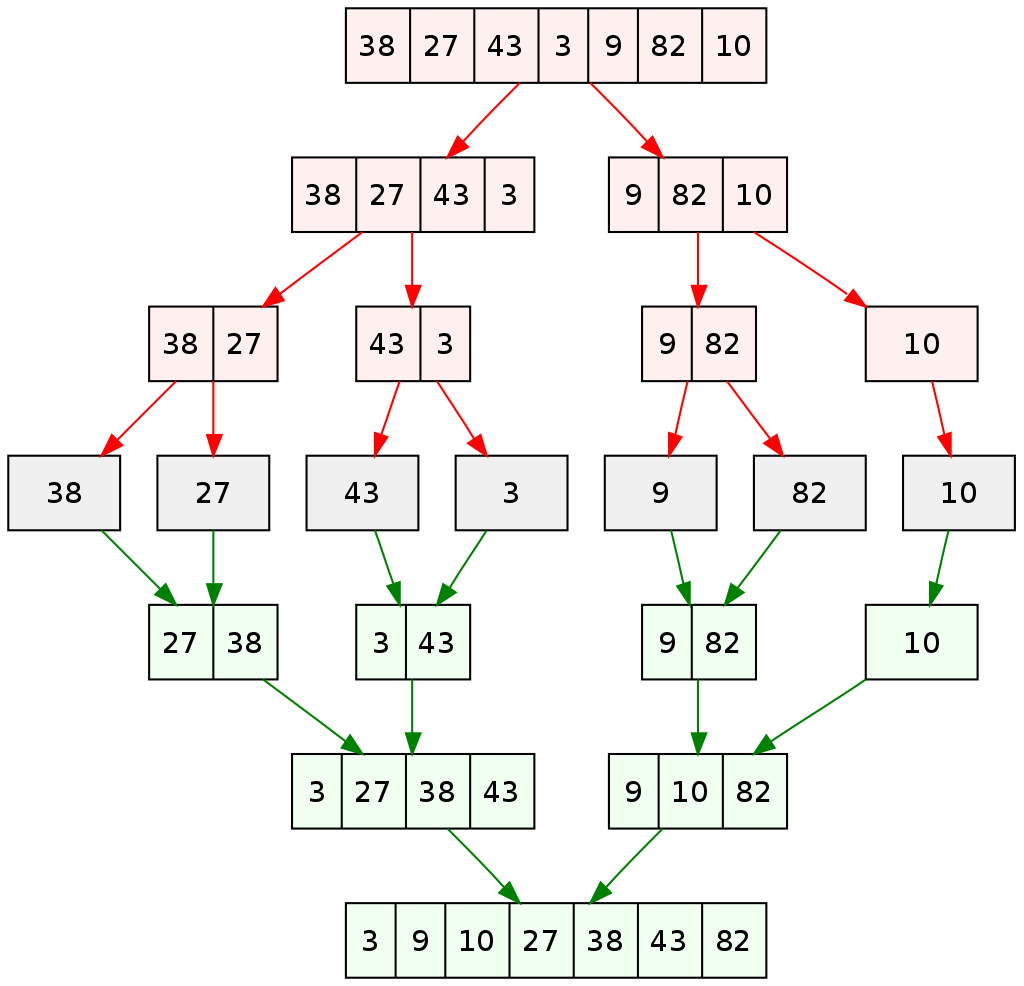
\includegraphics[width=10cm]{OperacionMergeSort.png}
        \caption{Ordenamiento de un arreglo de 7 valores enteros utilizando el algoritmo \textit{MergeSort}}
        \label{OperacionMergeSort}
    \end{figure}
    
\section*{Quick Sort}
    Quick Sort es un algoritmo basado en la técnica divide y vencerás creado por el científico británico C. A. R. Hoare, quién también es conocido como Tony Hoare, en el año de 1960.\\
    
    Es el algoritmo más ampliamente utilizado en el mundo para el ordenamiento numérico, también es considerado el algoritmo más eficiente y veloz de los métodos de ordenación interna.
    
    La complejidad del algoritmo para su caso promedio es O(nlogn), pero en su peor caso tendrá la complejidad O($n^2$), dandose este caso cuando el pivote queda en alguno de los extremos.
    
    El funcionamiento del algoritmo se describe en 4 pasos:\\
    \begin{enumerate}
        \item Se elige un elemento de la lista a ordenar, se le llamará pivote
        \item Se reacomodan los elementos de la lista según el valor de pivote, de manera que los elementos antes de este son siempre menores, y los que están después serán siempre mayores. Después de este ordenamiento parcial, el pivote ya se encuentra colocado en el lugar exacto que debe ocupar en la lista final.
        \item La lista se separa en 2 sublistas, una formada por los elementos a la izquierda del pivote, y otra por los elementos a su derecha.
        \item Se repite el proceso de forma recursiva para todas las sublistas mientras estas contengan más de un elemento. Al terminar este proceso todos los elemento se encuentran ordenados.
    \end{enumerate}
    
    En este algoritmo la elección del pivote es muy importante, pues dependiendo de la elección, el algoritmo puede ser más o menos eficiente. Si bien tomar un elemento cualquiera como pivote no requiere de cálculo alguno, la elección a ciegas puede provocar para ciertas entradas una complejidad de O($n^2$).\\
    
    Una alternativa para subsanar este problema es conocer de antemano el elemento central para utilizar como pivote, esta operación puede realizarse en O(n) y asegura hasta para el peor de los casos que el algoritmo sea O(nlogn), sin embargo este cálculo adicional rebaja la eficiencia en el caso promedio.\\
    
    Otra opción es tomar tres elementos de la lista, comúnmente se escoge el primero, medio y último elemento del arreglo, se comparan y el valor medio es escogido como el pivote.

\chapter*{Experimentación y Resultados}
    \section*{MergeSort}
        \hfill \break
\hfill \break
\hfill \break
\hfill \break
\hfill \break
\hfill \break
\hfill \break
\hfill \break
\hfill \break
\hfill \break

\subsection*{Algoritmo Merge}
    El algoritmo utilizado para la realización de esta práctica es en unos aspectos muy particulares diferentes al mostrado en clase. El código que se implementa como muestra utiliza un ciclo \textit{for} para realizar el ordenamiento de los 2 subarreglos obtenidos, más esta implementación ignora el tamaño de estos subarreglos, provocando que en las verificaciones del tamaño del valor de estos se utiliza un índice fuera de los límites, genrando una excepción. \\
    
    Para subsanar este inconveniente, se utiliza en cambio, un ciclo \textit{while} que iterará las variables que recorren los 2 subarreglos hasta que una de estas al menos, exceda el límite de los índices. \\
    
    Cuando se cumpla esta condición, existe la posibilidad de que alguna de las variables no alcancé el índice máximo, significando que no se ha recorrido por completo el subarreglo. Dado que es seguro que los valores restantes sin verificar en el subarreglo restante son los mayores, se procede únicamente mediante un ciclo \textit{while} que agote los valores recorridos y los vaya ingresando en el arreglo de retorno. \\
    
    El pseudocódigo de la implementación programada se muestra en la figura \ref{PseudocodigoMerge}:

    \begin{figure}[h!]
        \centering
        \begin{verbatim}
            int[] Merge(A[],p,q,r)
                n1 = q-p+1
                n2 = r-q
                
                # Creación e inicialización de los subarreglos
                L = new int[n1]
                R = new int[n2]
                for i=0 to i<n1 do
                    L[i] = A[p+i]
                for j=0 to j<n2 do
                    R[j] = A[q+j+1]
                
                # Inicia el ordenamiento de los valores en el arreglo de entrada A
                i = 0
                j = 0
                k = p
                while i<n1 and j<n2 do
                    if L[i] <= R[j]
                        A[k] = L[i]
                        i++
                    else
                        A[k] = R[j]
                        j++
                        
                # Se terminan de ingresar los valores de los subarreglos sin recorrer completamente   
                while i<n1 do
                    A[k] = L[i]
                    i++
                    k++
                while j<n2 do
                    A[k] = R[j]
                    j++
                    k++
                    
                return A
        \end{verbatim}
        \caption{Pseudocódigo del algoritmo Merge}
        \label{PseudocodigoMerge}
    \end{figure}
    
    \newpage
    
\hfill \break
\hfill \break
\hfill \break
\hfill \break

    \subsubsection*{Complejidad de \textbf{Merge} mediante gráficas}
        Para la obtención de los pares ordenados que se grafícaron, se realizó una evaluación del número de operaciones realizadas en el algoritmo para completar su flujo. Se utilizaron arreglos generados aleatoriamente con valores entre el 0 y el 9, y según las necesidades del algoritmo, se encuentran ordenados en 2 subarreglos. \\
        
        Se varía el tamaño del arreglo con la intención de obtener los valores que se graficarán. Estos valores se tomaron de 10 en 10, empezando desde el 1 y terminando en el 200, los puntos obtenidos se muestrán en la figura \ref{PuntosMerge}.\\
        
        \begin{figure}[h!]
            \centering
            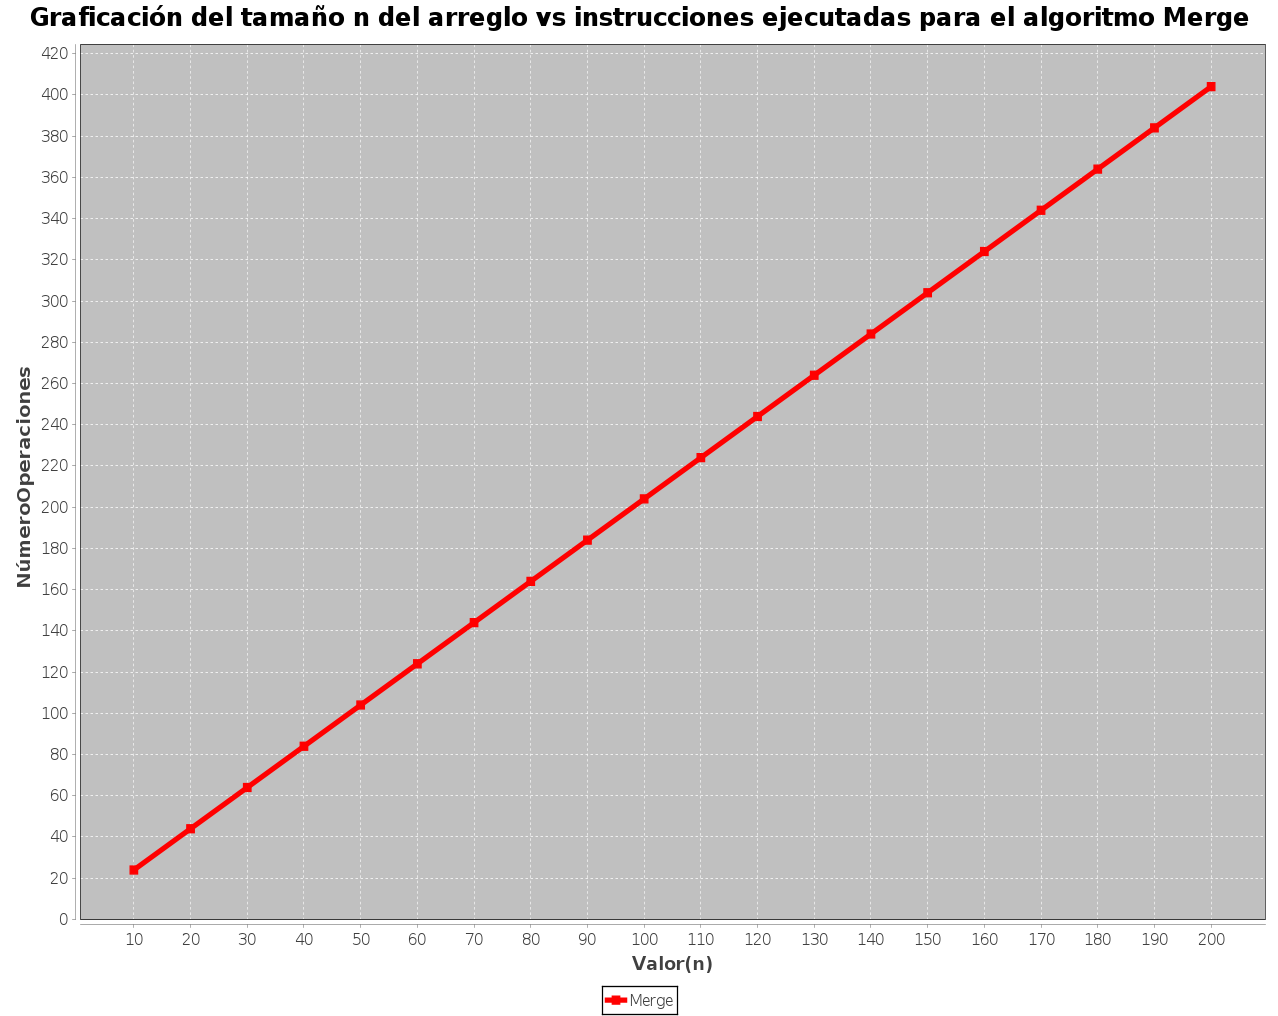
\includegraphics[width=19cm]{MergeSort/GraficaMerge.png}
            \caption{Representación gráfica de la complejidad del algoritmo Merge mediante la evaluación del número de instrucciones realizadas}
            \label{GraficaMerge}
        \end{figure}
        
        \begin{figure}[h!]
            \centering
            \begin{tabular}{c c}
            P0( 1,6 ) & \\
                P1( 10,24 ) & P11( 110,224 )\\
                P2( 20,44 ) & P12( 120,244 )\\
                P3( 30,64 ) & P13( 130,264 )\\
                P4( 40,84 ) & P14( 140,284 )\\
                P5( 50,104 ) & P15( 150,304 )\\
                P6( 60,124 ) & P16( 160,324 )\\
                P7( 70,144 ) & P17( 170,344 )\\
                P8( 80,164 ) & P18( 180,364 )\\
                P9( 90,184 ) & P19( 190,384 )\\
                P10( 100,204 ) & P20( 200,404 )\\
            \end{tabular}
            \caption{Pares ordenados obtenidos de la evaluación del algoritmo Merge}
            \label{PuntosMerge}
        \end{figure}
    
    Y la gráfica generada por estos pares se muestra en la figura \ref{GraficaMerge}.\\
    
    Se aprecia claramente en la gráfica una recta, implicando que la complejidad del algoritmo es lineal. A continuación se demuestra su relación con una ecuación lineal.\\
    
\hfill \break
\hfill \break
\hfill \break
\hfill \break

    La ecuación para la recta en su forma punto-pendiente es: \textbf{y=mx+b}
    Primero encontramos el término independiente, este término implica en el código operaciones de complejidad lineal, tales como asignaciones de variables.\\
    
    Tomaremos por facilidad, los puntos \textbf{P1} y \textbf{P2}:\\
    \begin{equation*}
        \begin{split}
            P1 \rightarrow 24= & 10m + b \\
            P2 \rightarrow 44= & 20m + b
        \end{split}
    \end{equation*}
    Se despeja la pendiente e igualan los términos:\\
    \begin{equation*}
        \begin{split}
            m= & \frac{24-b}{10} \\
            m= & \frac{44-b}{20} \\
            \\
            \frac{24-b}{10}= & \frac{44-b}{20}\\
            480-20b= & 440-10b\\
            40= & 10b\\
            b= & 4
        \end{split}
    \end{equation*}
    Ahora simplemente sustituimos el valor del término independiente en alguna de las 2 ecuaciones con la pendiente despejada:
    \begin{equation*}
        \begin{split}
            m=& \frac{24-4}{10}\\
            m=& \frac{20}{10}\\
            m=& 2
        \end{split}
    \end{equation*}
    Concluimos que los valores para el término independiente y la pendiente son:
    \begin{equation*}
        \begin{split}
            \textbf{m=} & \textbf{2}\\
            \textbf{b=} & \textbf{4}
        \end{split}
    \end{equation*}
    
    Obtenidos estos valores es fácil realizar la subsitución en la ecuación \ref{EcuacionLinealMerge} para comprobar que cualquier valor dado como tamaño \textbf{n}(correspondiente a \textbf{x}) nos dará un número de operaciones(correspondiente a \textbf{y}).
    \begin{figure}[h!]
        \centering
        \begin{equation*}
           \textbf{y=2x + 4}
        \end{equation*}
        \caption{Ecuación para el cálculo del número de operaciones realizadas en el algoritmo Merge para un tamaño \textbf{x} dado}
        \label{EcuacionLinealMerge}
    \end{figure}
    
    Se concluye entonces que:
    \begin{equation*}
        Merge(n) \in \Theta(n)
    \end{equation*}
    \newpage
    
    
    
    
    
    
    
    \subsubsection*{Complejidad de \textbf{Merge} analíticamente}
    
    Ahora nos apoyamos en el pseudocódigo \ref{PseudocodigoMerge} para el análisis por bloque de las instrucciones en la función Merge: \\
    
    El primer bloque analizado corresponde solamente a asignaciones, correspondiendoles una complejidad constante:
    \begin{equation*}
        \left.
            \begin{aligned}
                \text{n1 = q-p+1} \\
                \text{n = r-q} \\
                \text{L = new int[n1]} \\
                \text{R = new int[n2]}
            \end{aligned}
        \right\}
        \quad\Theta(1)
    \end{equation*}
    
    El siguiente bloque de instrucciones dan los valores a los subarreglos que deben de combinarse para integrarse en 1 solo ordenado:
    \begin{equation*}
        \left.
            \begin{aligned}
                \text{for i=0 to i}<\text{n1 do} \\
                \text{L[i] = A[p+1]} \\
                \text{for j=0 to j}<\text{n2 do}\\
                \text{R[j] = A[q+j+1]}
            \end{aligned}
        \right\}
        \quad\Theta(n)
    \end{equation*}
    
    Le sigue un bloque con asignaciones que son importantes para el correcto ordenamiento de los arreglos.
    La variable \textbf{i} representa el índice del subarreglo \textbf{L}.
    La variable \textbf{j} representa el índice del subarreglo \textbf{R}.
    La variable \textbf{k} representa el índice del arreglo origen \textbf{A}, y por lo tanto donde se realizarán las inserciones de valores ordenadamente. Esta variable se inicia en el valor de \textbf{p}, que es la posición del primer elemento que se ordena y por lo tanto también es la posición del primer elemento del subarreglo \textbf{L}:
    \begin{equation*}
        \left.
            \begin{aligned}
                \text{i = 0} \\
                \text{j = 0} \\
                \text{k = p}
            \end{aligned}
        \right\}
        \quad\Theta(1)
    \end{equation*}
    
    Inicia el ordenamiento de los valores que contiene \textbf{A} mediante la evaluación de los contenidos en los subarreglos:
    \begin{equation*}
        \left.
            \begin{aligned}
                \left.
                    \begin{aligned}
                        \text{while i}<\text{n1 and j}<\text{n2 do} \\
                        \text{if L[i] <= R[j]} \\
                        \text{A[k] = L[i]} \\
                        \text{i++} \\
                        \text{else} \\
                        \text{A[k] = R[j]} \\
                        \text{j++} \\
                    \end{aligned}
                \right\}
                \quad\Theta(n1+n2-c)
                \\
                \left.
                    \begin{aligned}
                        \left.
                            \begin{aligned}
                                \text{while i}<\text{n1 do}\\
                                \text{A[k] = L[i]}\\
                                \text{i++} \\
                                \text{k++}
                            \end{aligned}
                        \right\}
                        \quad \Theta(c_1)
                        \\
                        \left.
                            \begin{aligned}
                                \text{while i}<\text{n1 do}\\
                                \text{A[k] = R[j]}\\
                                \text{j++} \\
                                \text{k++}
                            \end{aligned}
                        \right\}
                        \quad \Theta(c_2)
                    \end{aligned}
                \right\}
                \quad\Theta(c)
            \end{aligned}
        \right\}
        \quad\Theta(n)
    \end{equation*}
    En el primer bloque observamos una complejidad \textbf{n1+n2-c}, esto implica que se recorren los subarreglos \textbf{L} y \textbf{R} hasta que se alcance el límite de uno de ellos, por esta razón se agrega una \textbf{c} constate que indica la diferencia de índices restantes para el subarreglo que aún no se ha agotado hasta el límite de sus valores.\\
    
    Por esta misma razón, los siguientes 2 bloques iterarán aumentando el valor de los índices de los 2 subarreglos hasta que los 2 ingresen todos los valores en A. Siempre se dará el caso donde solo 1 de estos \textit{while} iterará, mientras el otro solo realiza la verificación pero no ejecuta su interior. Las 2 constantes(\textbf{c1,c2}) pueden tomar el valor de 0 o \textbf{c}, resultandonos al realizar la suma de sus complejidades tan solo la constante \textbf{c}.\\
    
    Finalmente la complejidad de estos 3 bloques nos resulta: $n1+n2-c+c = n1+n2$
    Pero el valor de esta suma es igual al tamaño del arreglo \textbf{A} original, por lo que se concluye que el valor de ese bloque es lineal.\\
    
    La suma de las complejidades de los bloques nos queda de la siguiente manera:
    \begin{equation*}
        \Theta(1) + \Theta(n) + \Theta(1) + \Theta(n) = 2\Theta(n) + 2\Theta(1) = 2\Theta(n)
    \end{equation*}
    El 2 que multiplica a la complejidad lineal, es la constante encontrada en el análisis \textit{a posteriori} realizada en la sección anterior, sin embargo esta cifra nos es solamente útil si deseamos expresar una ecuación que acote de forma justa a la resultada por este algoritmo, no siendo el caso presente se concluye que:
    \begin{equation*}
        Merge(n) \in \Theta(n)
    \end{equation*}
    
    
    
    
\subsection*{Algoritmo MergeSort}
    Para la implementación de este algoritmo se utilizó el mismo código mostrado en el video. Contiene pocas líneas de código y es bastante claro en su funcionamiento, pero es gracias a la utilización del algoritmo \textbf{Merge} que este funciona enteramente como divisor de subproblemas, y que mediante \textbf{Merge} se irán uniendo para integrar y obtener el ordenamiento de todo el arreglo. \\
    
    El pseudocódigo de este se muestra en la siguiente figura \ref{CodigoMergeSort}:
    \begin{figure}[!h]
        \centering
        \begin{verbatim}
            int[] MergeSort(A[],p,r)
                if p<r
                    q = (p+r)/2
                    
                    MergeSort(A,p,q)
                    MergeSort(A,q+1,r)
                    Merge(A,p,q,r)
                    
                    return A
        \end{verbatim}
        \caption{Pseudocódigo del algoritmo MergeSort}
        \label{PseudocodigoMergeSort}
    \end{figure}
    
    \subsubsection*{Complejidad de \textbf{MergeSort} mediante gráficas}
    
    Para la obtención de los pares ordenados que se grafícaron, se realizó una evaluación del número de operaciones realizadas en el algoritmo para completar su flujo. Se utilizaron arreglos generados aleatoriamente con valores entre el 0 y el 9.
        
        Se varía el tamaño del arreglo con la intención de obtener los valores que se graficarán. Estos valores se tomaron de 10 en 10, empezando en el 1 y terminando en el 200, los puntos obtenidos se muestrán en la figura \ref{PuntosMergeSort}.\\
        
        \begin{figure}[h!]
            \centering
            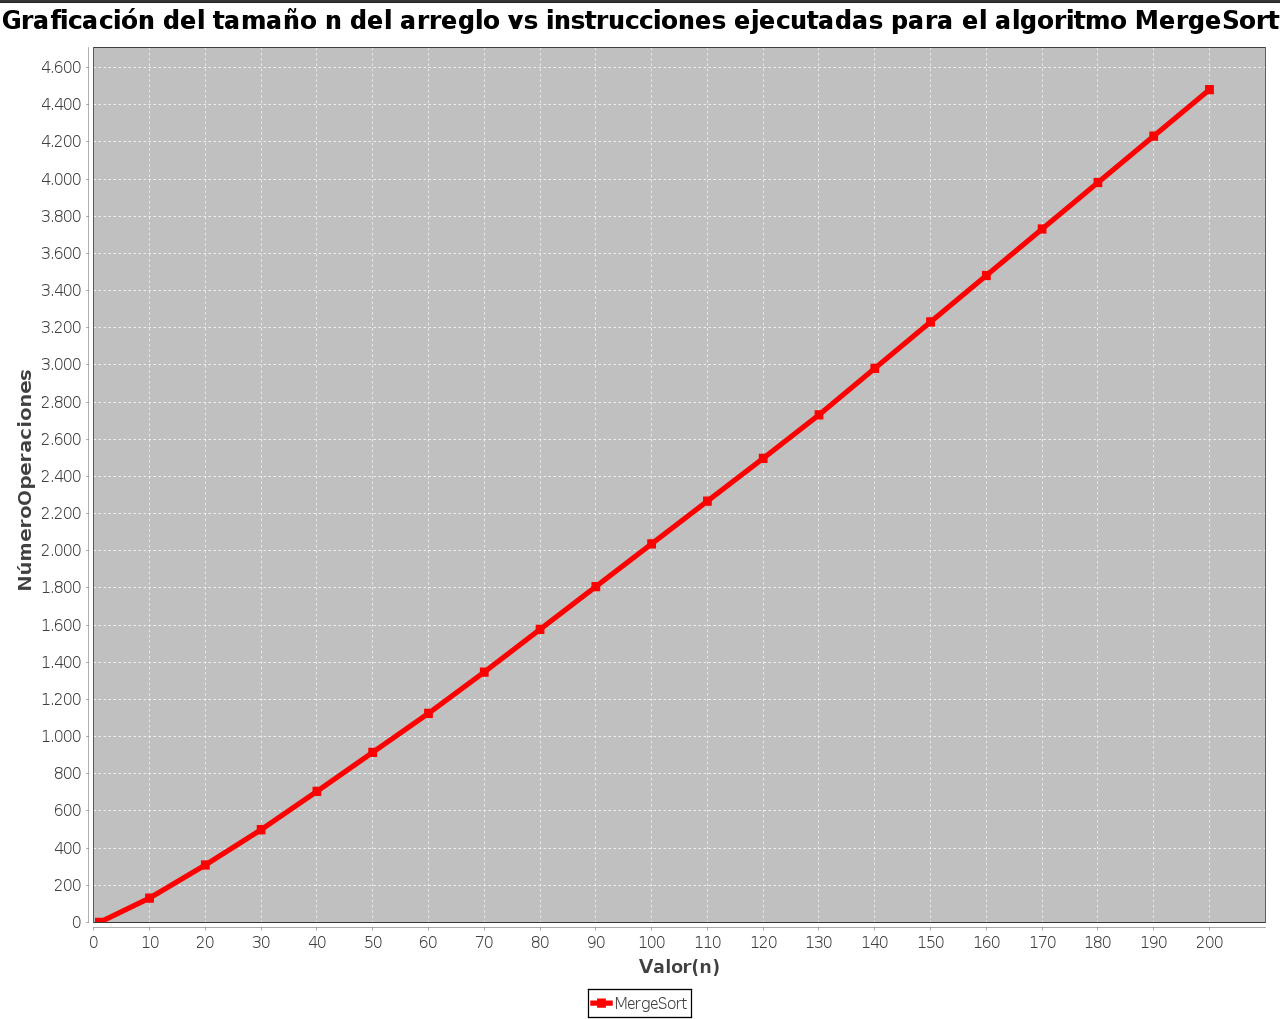
\includegraphics[width=17cm]{MergeSort/GraficaMergeSort.png}
            \caption{Representación gráfica de la complejidad del algoritmo MergeSort mediante la evaluación del número de instrucciones realizadas}
            \label{GraficaMergeSort}
        \end{figure}
        
        \begin{figure}[h!]
            \centering
            \begin{tabular}{c c}
                P0( 1, 0 ) & \\
                P1( 10,131 ) & P11( 110,2267 )\\
                P2( 20,309 ) & P12( 120,2497 )\\
                P3( 30,499 ) & P13( 130,2731 )\\
                P4( 40,705 ) & P14( 140,2981 )\\
                P5( 50,915 ) & P15( 150,3231 )\\
                P6( 60,1125 ) & P16( 160,3481 )\\
                P7( 70,1347 ) & P17( 170,3731 )\\
                P8( 80,1577 ) & P18( 180,3981 )\\
                P9( 90,1807 ) & P19( 190,4231 )\\
                P10( 100,2037 ) & P20( 200,4481 )\\
            \end{tabular}
            \caption{Pares ordenados obtenidos de la evaluación del algoritmo Merge}
            \label{PuntosMergeSort}
        \end{figure}
    
    Y la gráfica generada por estos pares se muestra en la figura \ref{GraficaMerge}.\\
    
    Aparentemente, dado el primer vistazo pareciera ser una gráfica generada por la ecuación de una recta, pero se tiene una particularidad en el \textbf{P0}, donde para el valor de la unidad en el tamaño del arreglo, y en el caso del análisis que sería para el valor de la \textbf{x}, se obtiene el valor 0. Si se evaluara tal valor en la ecuación \textbf{y=mx+b}, obtendríamos un valor definitivamente mayor a 0. \\
    
    Debido a esto podemos descartar una complejidad lineal para el algoritmo, pues no existe un valor para la pendiente \textbf{m} y para la constante \textbf{b} que al sustituir nos describa los puntos obtenidos. Así entonces y considerando según la jerarquía de cotas una superior a la complejidad lineal. \\
    
    La cota mayor inmediata es el \textbf{nlogn}, tal que ahora se muestran gráficas en la figura \ref{GraficasPropuestaMergeSort}, que comparan el comportamiento de la obtenido por el algoritmo y las 2 ecuaciones consideradas hasta el momento:\\
    
    \begin{figure}[h!]
        \centering
        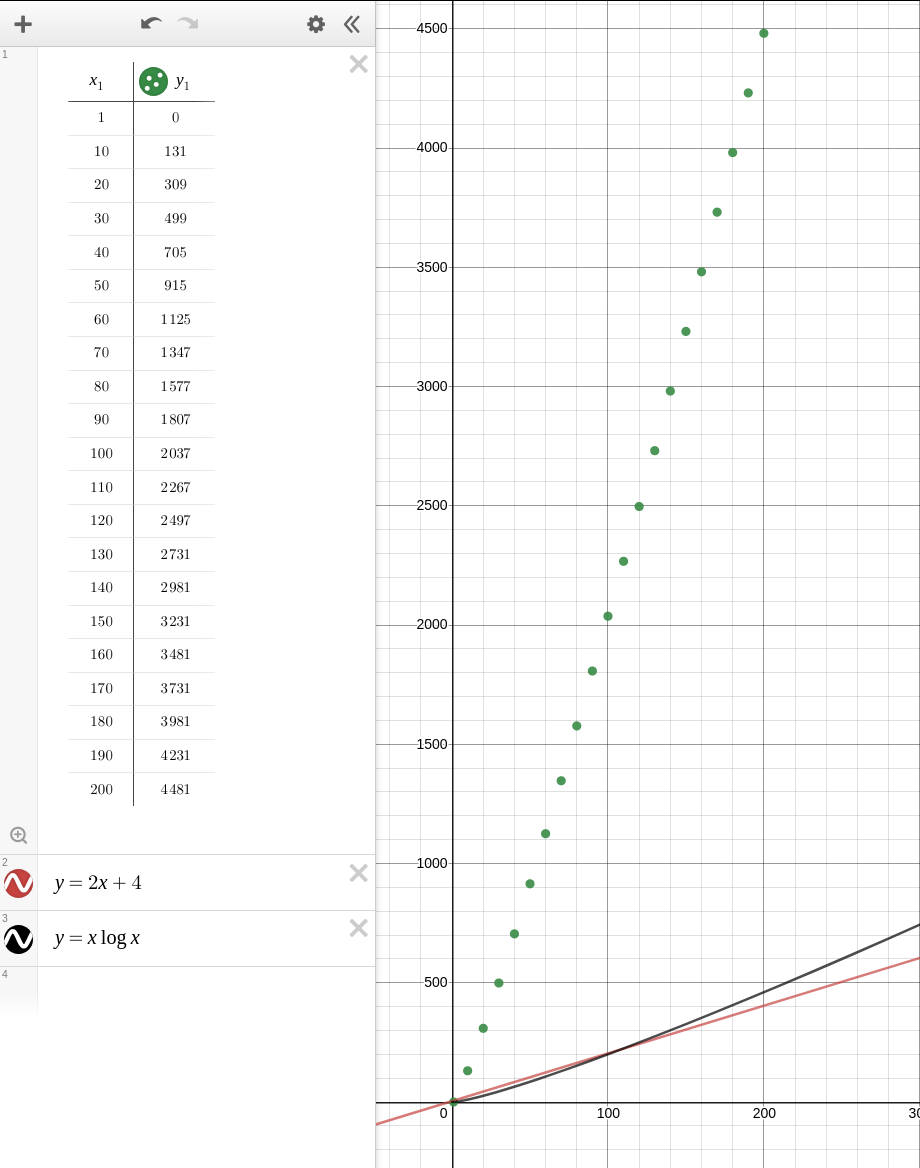
\includegraphics[width=15cm]{MergeSort/GraficasPropuestaMergeSort.png}
        \caption{Los puntos verdes corresponden a los obtenidos en la evaluación del algoritmo.\\ La gráfica en color rojo corresponde a la ecuación que describe la complejidad obtenido para el algoritmo \textbf{Merge}.\\ La gráfica en color negro corresponde a la cota propuesta para la complejidad de \textbf{MergeSort}}
        \label{GraficasPropuestaMergeSort}
    \end{figure}
    
    \hfill \break
    \hfill \break
    \hfill \break
    \hfill \break
    \hfill \break
    
    Hasta este momento en la figura \ref{GraficasPropuestaMergeSort} tan solo es visible que ciertamente la ecuación \textbf{xlogx} tiende a crecer más rápidamente que la ecuación lineal a partir de un valor de \textbf{x}, pero evidentemente esta ecuación crece mucho más lento que lo que hace la obtenida por nuestro análisis del algoritmo. Para acortar esta brecha entre las 2, se propone entonces agregar una constante que multiplique a la ecuación tal como lo muestra la figura \ref{GraficasFinalesMergeSort}.
    
    \begin{figure}[h!]
        \centering
        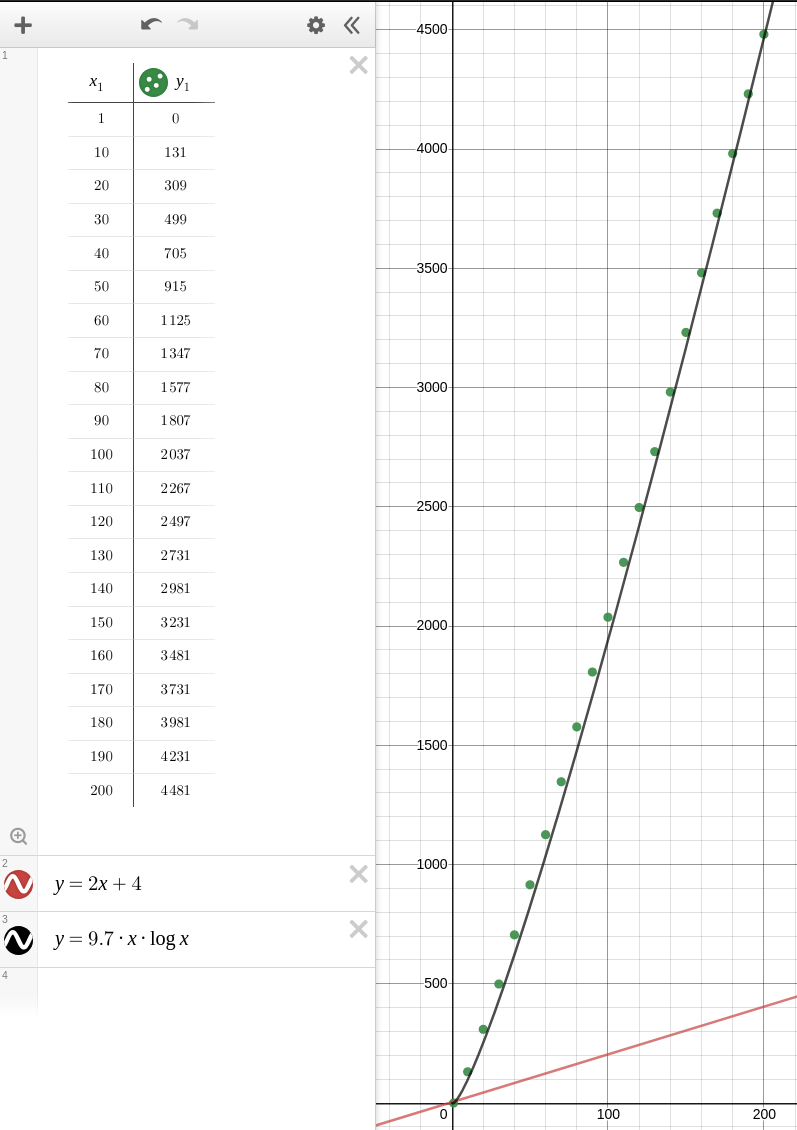
\includegraphics[width=13cm]{MergeSort/GraficasFinalesMergeSort.png}
        \caption{Los puntos verdes corresponden a los obtenidos en la evaluación del algoritmo.\\ La gráfica en color rojo corresponde a la ecuación que describe la complejidad obtenido para el algoritmo \textbf{Merge}.\\ La gráfica en color negro corresponde a la cota propuesta para la complejidad de \textbf{MergeSort}}
        \label{GraficasFinalesMergeSort}
    \end{figure}
    \newpage
    
    La asignación de la constante multiplicativa fue asignada de forma arbritaria a la que más justamente se acomodaba a la trayectoria de los puntos, esto con el único fin de mostrar que existe una posible \textbf{c} constante que multiplique a la ecuación para describir exactamente al comportamiento del algoritmo, y de esta forma nos es posible concluir que la complejidad del algoritmo \textbf{MergeSort} es:
    \begin{equation*}
        \text{MergeSort} \in \Theta(nlogn)
    \end{equation*}
    
    \newpage
    
    \subsubsection*{Complejidad de \textbf{MergeSort} analíticamente}
        Retomamos la figura \ref{PseudocodigoMergeSort} que contiene el pseudocódigo de la función, y se inicia el análisis por bloques de la función:
    \begin{equation*}
        \left.
            \begin{aligned}
                \bigl.
                    \text{if p}<r
                \bigr\}
                \quad\Theta(1)
                \\
                \bigl.
                    \text{q = (p+r)/2}
                \bigr\}
                \quad\Theta(1)
                \\
                \bigl.
                    \text{MergeSort(A,p,q)}
                \bigr\}
                \quad\text{M}\left(\frac{n}{2}\right)
                \\
                \bigl.
                    \text{MergeSort(A,q+1,r)}
                \bigr\}
                \quad\text{M}\left(\frac{n}{2}\right)
                \\
                \bigl.
                    \text{Merge(A,p,q,r)}
                \bigr\}
                \quad\Theta(n)
            \end{aligned}
        \right\}
        \quad2\text{M}\left(\frac{n}{2}\right)+\Theta(n)
    \end{equation*}
    
    De donde vamos a considerar a \textbf{M(n)} como la ecuación de recursividad en \ref{EcuacionRecursivaMergeSort}:
    \begin{figure}[h!]
        \centering
        \begin{equation*}
            M(n)=2M \left( \frac{n}{2} \right) +\Theta(n)
        \end{equation*}
        \caption{Ecuación de recursividad para el algoritmo MergeSort}
        \label{EcuacionRecursivaMergeSort}
    \end{figure}
    
    De la ecuación se idenfican:\\
    $a = 2$\\
    $b = 2$\\
    $f(n) = cn$
    
    Con los elementos identificados de la ecuación, evaluamos para obtener la complejidad usando el \textit{Método maestro}.\\
    Como primer paso obtenemos los valores de la siguiente ecuación:
    \begin{equation*}
        n^{log_ba} = n^{log2} = n
    \end{equation*}
    
    Y verificamos con respecto a \textbf{f(n)}:
    \begin{equation*}
        n = n^{log_ba} = f(n) = n
    \end{equation*}
    
    Dado que esto se cumple, obtenemos la complejidad mediante el caso \textbf{II} del Teorema maestro:
    \begin{equation*}
        M(n) \in \Theta(n^{log_ba}logn) \Rightarrow M(n) \in \Theta(nlogn)
    \end{equation*}

        \newpage
    
    \section*{QuickSort}
        \hfill \break
\subsection*{Algoritmo Partition}
    La función clave en QuickSort es Partition(). El objetivo de esta función es, dado un arreglo toma como "pivote" al ultimo elemento del arreglo y pone al elemento tomado como pivote en la posición correcta del arreglo. Pone a los elementos menores al pivote a su izquierda y aquellos mayores a su derecha.
    
    El pseudocódigo  del algoritmo se muestra en la figura \ref{PseudocodigoPartition}:
    
    \begin{figure}[h!]
        \centering
        \begin{verbatim}
            int Partition(int A[], int prim, int ult)
                int pivote = A[ult]
                int i=prim-1
                for j=prim to j<ult do 
                    if A[j]<pivote 
                        i++
                        # Se ejecuta un exchange
                        int tmp = A[i]
                        A[i]=A[j]
                        A[j]=tmp
                # Exchange
                int tmp=A[i+1]
                A[i+1]=A[ult]
                A[ult]=tmp
                return i+1
        \end{verbatim}
        \caption{Pseudocódigo de la función Partition}
        \label{PseudocodigoPartition}
    \end{figure}
    
    \subsection*{Complejidad de \textbf{Partition} mediante gráficas}
        Para la generación de nuestras gráficas, se realizó un conteo del número de operaciones realizadas en el algoritmo por cada entrada de arreglo de tamaño n. Se utilizaron arreglos generados aleatoriamente con valores entre el 0 y el 9. EL tamaño del arreglo de entrada se modifica con la intención de obtener puntos graficables. Los puntos se muestran en la figura \ref{PuntosPartition}.\\
        
        \begin{figure}[h!]
            \centering
            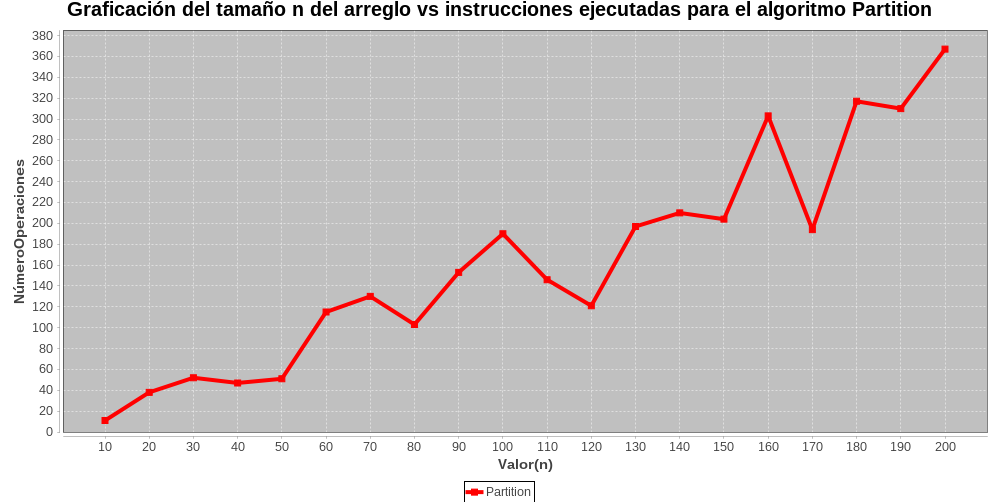
\includegraphics[width=13cm]{QuickSort/graf-partition.png}
            \caption{Representación gráfica de la complejidad temporal del algoritmo Partition, mediante la evaluación del número de instrucciones realizadas.}
            \label{GraficaPartition}
        \end{figure}
        
        \begin{figure}[h!]
            \centering
            \begin{tabular}{c|c}
                    P1( 10,11 ) & P11( 110,146 )\\
                    P2( 20,38 ) & P12( 120,121 )\\
                    P3( 30,52 ) & P13( 130,197 )\\
                    P4( 40,47 ) & P14( 140,210 )\\
                    P5( 50,51 ) & P15( 150,204 )\\
                    P6( 60,115 ) & P16( 160,303 )\\
                    P7( 70,130 ) & P17( 170,194 )\\
                    P8( 80,103 ) & P18( 180,317 )\\
                    P9( 90,153 ) & P19( 190,310 )\\
                    P10( 100,190 ) & P20( 200,367 )\\
            \end{tabular}
            \caption{Pares obtenidos de la evaluación del algoritmo Partition}
            \label{PuntosPartition}
        \end{figure}
        
        La gráfica generada por estos pares se muestra en la figura \ref{GraficaPartition}. Podemos apreciar que existe una dispersión de puntos que al contrario del algoritmo Merge no forman un patrón claro de recta, sin embargo, por las posiciones de los puntos podemos notar que pueden quedar acotados por una función lineal. A continuación, en la figura \ref{GraficaDesmosPartition} se propone la recta $y=2x$ y se considera la ecuación que describe la complejidad conocida para el algoritmo Partition como $y=x$.
        
        \begin{figure}[h!]
            \centering
            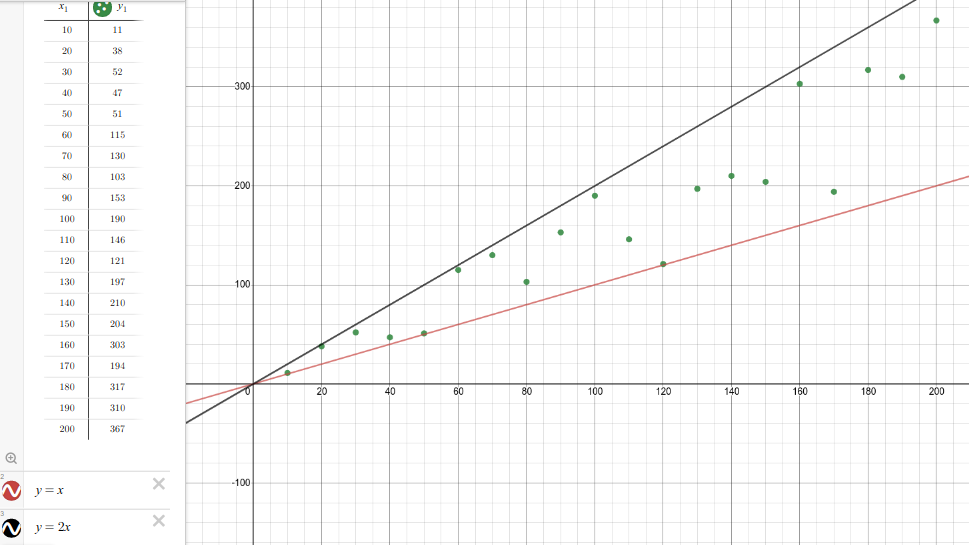
\includegraphics[width=13cm]{QuickSort/desmos-partition.png}
            \caption{Gráfica con función propuesta para acotar la complejidad de \textbf{Partition}. \\Los puntos verdes corresponden a los pares obtenidos en la evaluación del algoritmo. La recta en color negro corresponde a la ecuación conocida que describe la complejidad para el algoritmo \textbf{Partition}. La recta en color rojo corresponde a la cota propuesta para la complejidad de \textbf{Partition}.}
            \label{GraficaDesmosPartition}
        \end{figure}
        
        Para la eleccion de la constante multiplicativa de la cota propuesta en la figura \ref{GraficaDesmosPartition}, fue tomada al probar diversos valores y considerar que $y=2x$ era la que mejor se ajustaba en nuestro caso.
        
        
    \subsection*{Complejidad de \textbf{Partition} analíticamente}
        Para el cálculo analitico de la complejidad, retomaremos el pseudocódigo descrito en la figura \ref{PseudocodigoPartition}.
        
        \begin{equation*}
            \left.
                \begin{aligned}
                    \left.
                        \begin{aligned}
                            \text{pivote = A[ult]} \\
                            \text{i = prim-1} \\
                        \end{aligned}   
                    \right\}
                    \quad\Theta(1)
                    \\
                    \left.
                        \begin{aligned}
                            \text{for j=prim to j}<\text{ult do} \\
                            \text{if A[j]}<\text{pivote} \\
                            \text{int tmp=A[i]} \\
                            \text{A[i]=A[j]} \\
                            \text{A[j]=tmp} \\
                        \end{aligned}
                    \right\}
                    \quad\Theta(n)
                    \\
                    \left.
                        \begin{aligned}
                            \text{int tmp=A[i+1]} \\
                            \text{A[i+1]=A[ult]} \\
                            \text{A[ult]=tmp} \\
                            \text{return i+1} \\
                        \end{aligned}
                    \right\}
                    \quad\Theta(1)
                \end{aligned}
            \right\}
            \quad\Theta(n)
        \end{equation*}
        En el primer bloque encontramos una complejidad $\Theta(1)$ debido a que únicamente encontramos asignaciones a variables. Posteriormente, encontramos la complejidad del siguiente bloque que es $\Theta(n)$ que corresponde al bloque definido por el ciclo for que posiciona el pivote en el lugar correcto dentro del arreglo. Finalmente, el último bloque tiene una complejidad constante $\Theta(1)$ debido a que únicamente se ejecutan instrucciones que no pertenecen a ningún ciclo. Finalmente, se concluye que el algoritmo Partition posee una complejidad temporal lineal definida por $\Theta(n)$.
        
    \subsection*{Complejidad de \textbf{QuickSort} mediante gráficas}
        Para la generación de nuestras gráficas, se realizó un conteo del número de operaciones realizadas en el algoritmo por cada entrada de arreglo de tamaño n. Se utilizaron arreglos generados aleatoriamente con valores entre el 0 y el 9. EL tamaño del arreglo de entrada se modifica con la intención de obtener puntos graficables. Los puntos se muestran en la figura \ref{PuntosQSort}.\\
        
        \begin{figure}[h!]
            \centering
            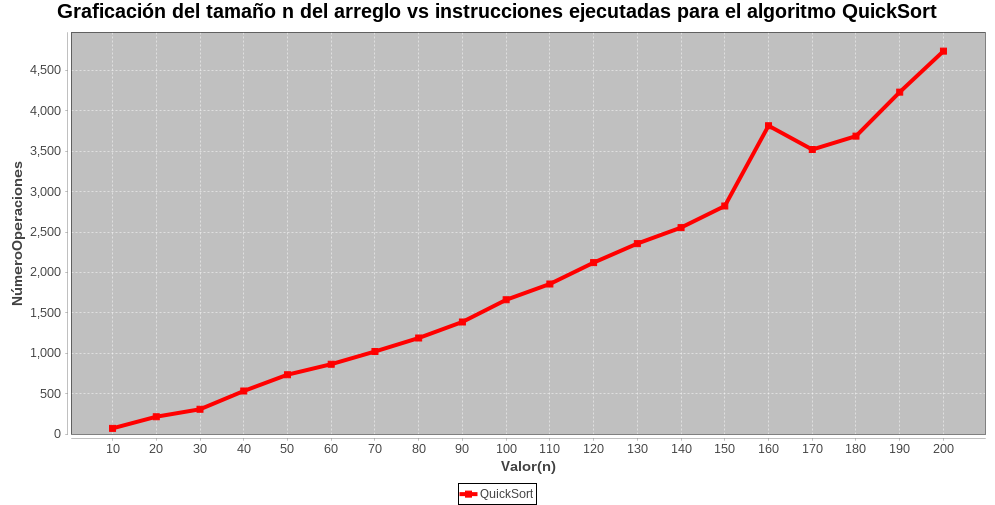
\includegraphics[width=13cm]{QuickSort/graf-qsort.png}
            \caption{Representación gráfica de la complejidad temporal del algoritmo \textbf{QuickSort}, mediante la evaluación del número de instrucciones realizadas.}
            \label{GraficaQSort}
        \end{figure}
        
        \begin{figure}[h!]
            \centering
            \begin{tabular}{c|c}
                    P1( 10,70 ) & P11( 110,1857 )\\
                    P2( 20,214 ) & P12( 120,2121 )\\
                    P3( 30,306 ) & P13( 130,2357 )\\
                    P4( 40,532 ) & P14( 140,2555 )\\
                    P5( 50,734 ) & P15( 150,2822 )\\
                    P6( 60,864 ) & P16( 160,3816 )\\
                    P7( 70,1021 ) & P17( 170,3521 )\\
                    P8( 80,1188 ) & P18( 180,3687 )\\
                    P9( 90,1387 ) & P19( 190,4232 )\\
                    P10( 100,1661 ) & P20( 200,4739 )\\
            \end{tabular}
            \caption{Pares obtenidos de la evaluación del algoritmo \textbf{QuickSort}}
            \label{PuntosQSort}
        \end{figure}
        
        La gráfica generada por estos pares se muestra en la figura \ref{GraficaQSort}. Es posible observar que el algoritmo muestra un ligero  patrón cuadrático de crecimiento. Debemos recordar que la funcion \textbf{Partition} divide al arreglo en dos subarreglos, sin embargo, no tenemos control del valor del pivote tomado por \textbf{Partition}.
        
        \begin{figure}[h!]
            \centering
            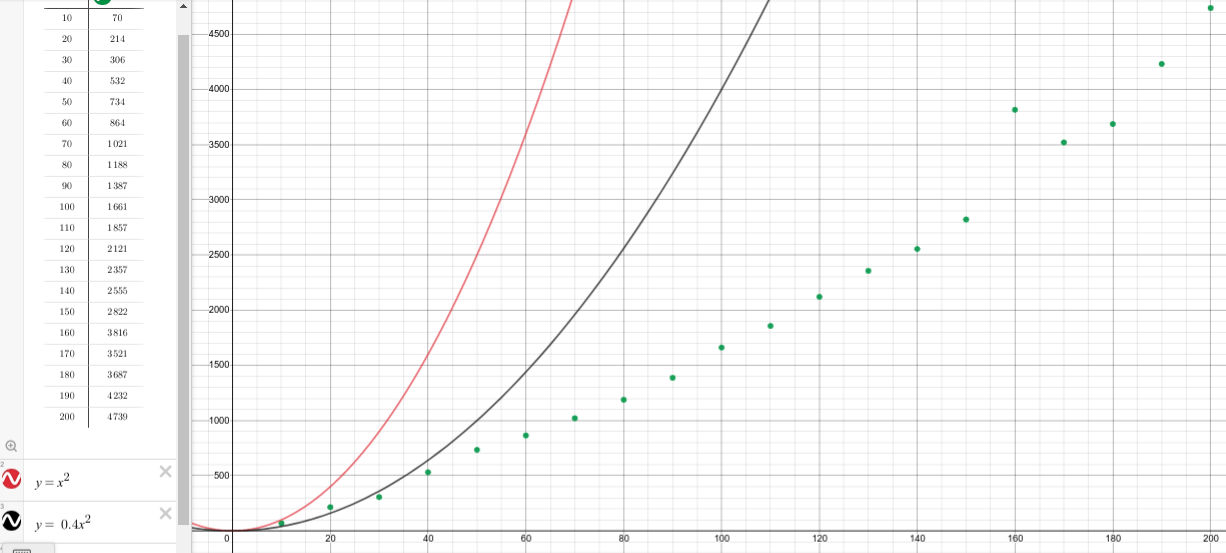
\includegraphics[width=17.5cm]{QuickSort/desmos-QSort.png}
            \caption{Gráfica con función propuesta para acotar la complejidad de \textbf{QuickSort}. \\Los puntos verdes corresponden a los pares obtenidos en la evaluación del algoritmo. La recta en color rojo $y=x^{2}$ corresponde a la ecuación conocida que describe la complejidad para el algoritmo \textbf{QuickSort}. La recta en color negro $y=0.4x^{2}$ corresponde a la cota propuesta para la complejidad de \textbf{QuickSort}.}
            \label{GraficaDesmosQSort}
        \end{figure}
        
        En la figura \ref{GraficaDesmosQSort} se propone como cota para el algoritmo a $y=x^{2}$ de acuerdo a los pares ordenados que se obtuvieron en la evaluación, 
        
    \subsection*{Complejidad de \textbf{QuickSort} analíticamente}
        Para el cálculo de la complejidad del algoritmo QuickSort consideraremos su pseudocódigo descrito en la figura \ref{PseudocodigoQSort}.
        
        \begin{figure}[h!]
        \centering
        \begin{verbatim}
            int[] QuickSort(A[], int prim, int ult)
                if prim < ult
                    int p = Partition(A, prim, ult)
                    QuickSort(A, prim, p-1)
                    QuickSort(A, p+1, ult)
                return A
        \end{verbatim}
        \caption{Pseudocódigo de la función QuickSort}
        \label{PseudocodigoQSort}
        \end{figure}
        
        Cuando el pivote divide el arreglo por la mitad, encontramos el mejor caso para el algoritmo QuickSort.
        
        \begin{equation*}
            \left.
                \begin{aligned}
                    \left.
                        \begin{aligned}
                            \text{q=Partition(A, prim, ult)}
                        \end{aligned}
                    \right\}
                    \quad\Theta(n)
                    \\
                    \left.
                        \begin{aligned}
                            \text{QuickSort(A, prim, q-1)}
                        \end{aligned}
                    \right\}
                    \quad T(q)
                    \\
                    \left.
                        \begin{aligned}
                            \text{QuickSort(A, q+1, n)}
                        \end{aligned}
                    \right\}
                    \quad T(n-q)
                    \\
                \end{aligned}
            \right\}
            \quad T(n) = T(q) + T(n-q) + \Theta(n)
        \end{equation*}
        
        De tal forma, se considerara \textbf{q=$\frac{n}{2}$}, y sustituimos en la ecuación de recurrencia:
        $T(n) = T(q)+T(n-q)+\Theta(n) \text{ Donde \textbf{q}, es la posición del pivote en el arreglo}$
                
        \begin{equation*}
            T(n)=T\left(\frac{n}{2}\right)+T\left(n-\frac{n}{2}\right)+\Theta(n) =2T\left(\frac{n}{2}\right)+\Theta(n)
        \end{equation*}
            
        Identificamos los elementos de la ecuacion:\\
        $a=2$\\
        $b=2$\\
        $f(n)=\Theta(n) = cn$\\
        Y procedemos a evaluar los requisitos del problema maestro:
        \begin{equation*}
            n^{log_ba}=n^{log2}=n
        \end{equation*}
        Se verifica entonces con respecto a \textbf{f(n)}:
        \begin{equation*}
            n=n^{log_ba}=f(n)=n
        \end{equation*}
            
        Por lo tanto, mediante el caso \textbf{II} del teorema maestro:
        \begin{equation*}
            T(n) = \Theta (n^{log_ba}logn) = \Theta(nlogn)
        \end{equation*}
        
    \subsection*{Proposición de orden de complejidad para \textbf{QuickSort} cuando todos los elementos del arreglo son distintos y están ordenados en forma decreciente.}
        
        En la figura \ref{GraficaQSortOrdenados} podemos observar el comportamiento del algoritmo teniendo como entrada un arreglo con todos los elementos distintos y ordenados de forma decreciente, para la generación de la gráfica consideramos el conteo de instrucciones ejecutadas.
        
        \begin{figure}[h!]
            \centering
            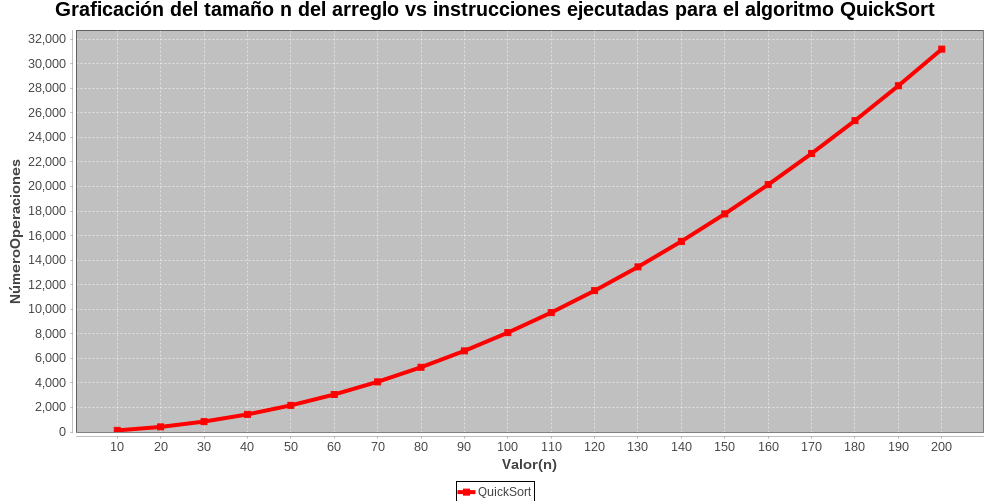
\includegraphics[width=13cm]{QuickSort/graf-qsort-ordenados.png}
            \caption{Representación gráfica de la complejidad temporal del algoritmo \textbf{QuickSort}, mediante la evaluación del número de instrucciones realizadas.}
            \label{GraficaQSortOrdenados}
        \end{figure}
        
        \begin{figure}[h!]
            \centering
            \begin{tabular}{c|c}
                    P1( 10,129 ) & P11( 110,9729 )\\
                    P2( 20,414 ) & P12( 120,11514 )\\
                    P3( 30,849 ) & P13( 130,13449 )\\
                    P4( 40,1434 ) & P14( 140,15534 )\\
                    P5( 50,2169 ) & P15( 150,17799 )\\
                    P6( 60,3054 ) & P16( 160,20154 )\\
                    P7( 70,4089 ) & P17( 170,22689 )\\
                    P8( 80,5274 ) & P18( 180,25374 )\\
                    P9( 90,6609 ) & P19( 190,28209 )\\
                    P10( 100,8094 ) & P20( 200,31194 )\\
            \end{tabular}
            \caption{Pares obtenidos de la evaluación del algoritmo \textbf{QuickSort} para el caso en que los elementos del arreglo son distintos y están ordenados de forma descendente.}
            \label{PuntosQSort}
        \end{figure}
        
        \begin{figure}[h!]
            \centering
            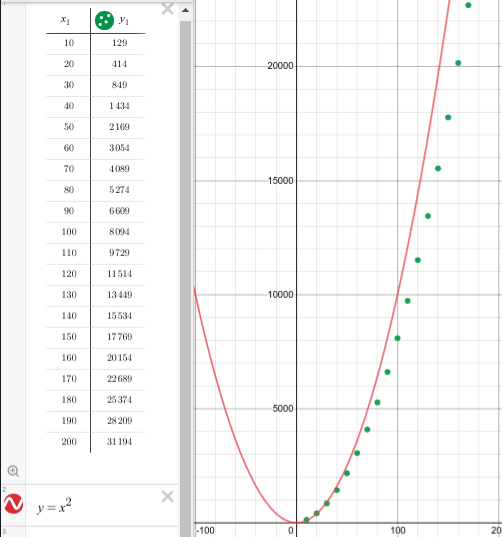
\includegraphics[width=13cm]{QuickSort/desmos-qsort-ordenado.png}
            \caption{Gráfica con función propuesta para acotar la complejidad de \textbf{Quicksort}. \\Los puntos verdes corresponden a los pares obtenidos en la evaluación del algoritmo. La función roja, es nuestra propuesta de cota superior para la complejidad temporal para el algoritmo Quicksort en su peor caso.}
            \label{GraficaDesmosPartition}
        \end{figure}
        
        Finalmente, podemos concluir que hemos comprobado gracias a nuestro analisis a posteriori, que el algoritmo posee una complejidad cuadrática para su peor caso.
        

        
\chapter*{Conclusiones}
    \begin{tabular}{l l}
        \multirow{3}{*}{
\includegraphics[width=1.5cm]{Imagenes/imanol.jpg}} &  \\
        & \textbf{Rivero Ronquillo Omar Imanol}\\
        & \\
    \end{tabular}
    \vspace*{3\baselineskip}\\
    Nunca había pensado en las formas en las que se podría optimizar la solución a un problema por medio de un algoritmo programable. Me pareció un enfoque increíble y ahora me parece que tengo claro porque se usan estos algorimos y en qué problemas se les podría dar un uso. A pesar de que en comparación con las prácticas anteriores se tuvieron que incluir más cosas además de los algorimos, para poder probarlos y estudiarlos, me parecieron un gran complemento en mi formación académica.
    
    En conclusión, me gustaría conocer más algoritmos de este tipo, me interesaron especialmente los algoritmos de compresión, aunque puedo estar bastante seguro de que las compresiones modernas deberán de tener una complejidad mayor de aprenderse y comprender su funcionamiento, que seguramente justificaran todo esto con las tasas de compresiones que puedan lograr.
    \\\\
    \begin{tabular}{l l}
        \multirow{3}{*}{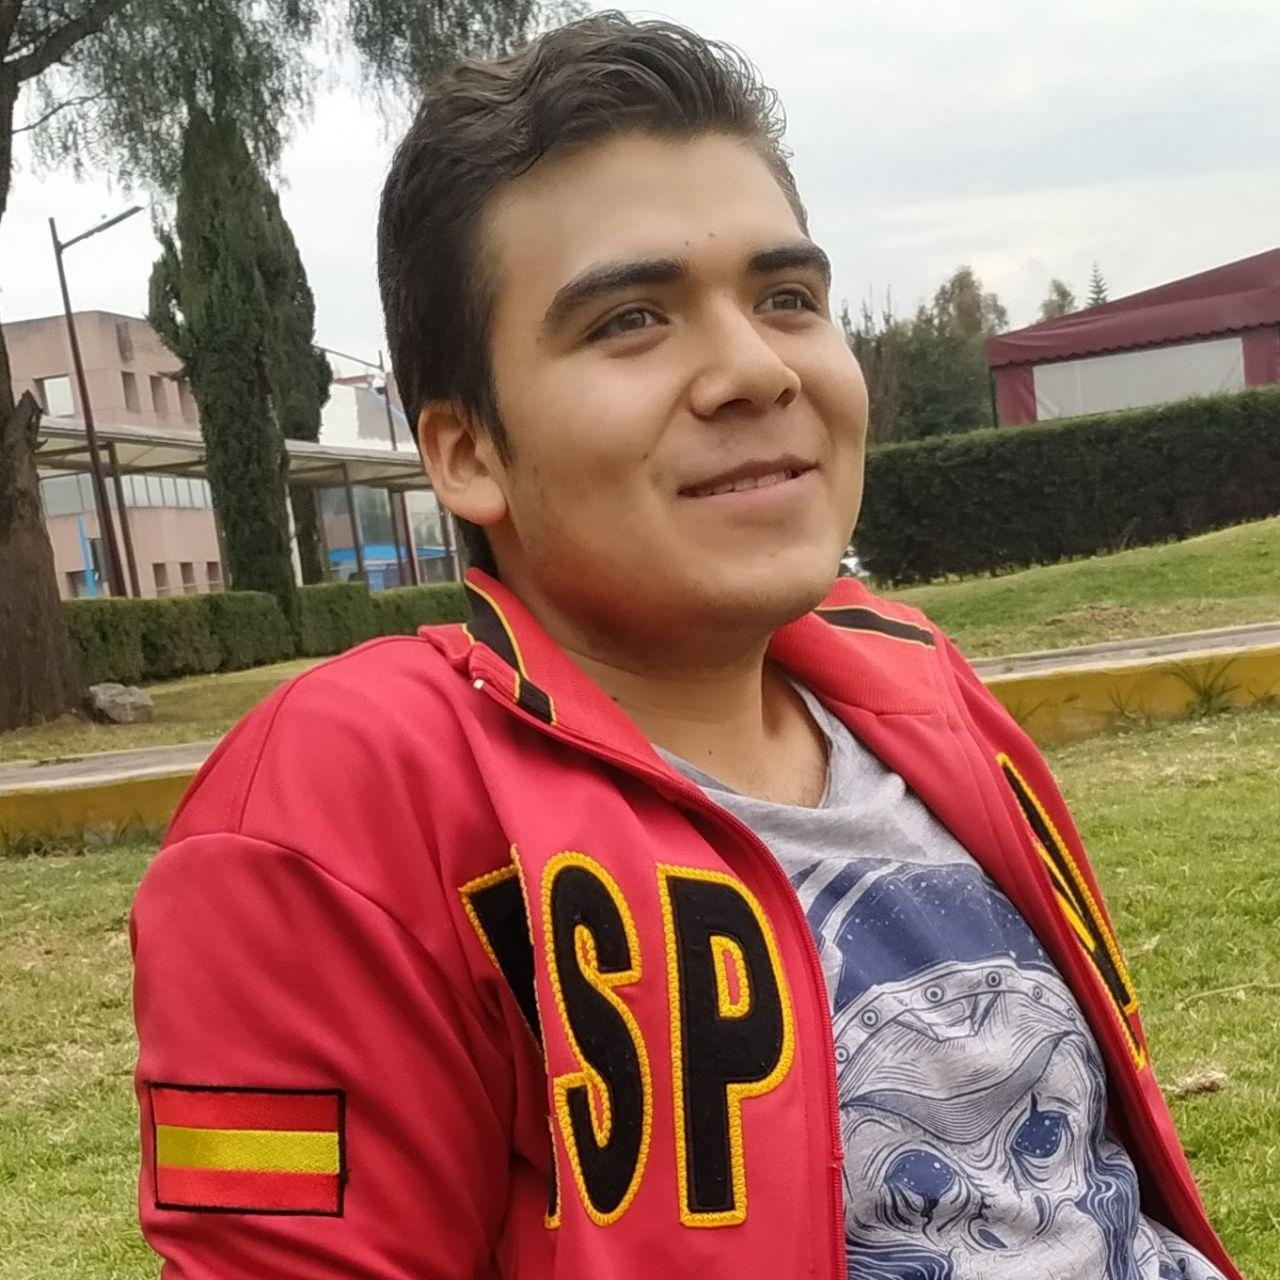
\includegraphics[width=1.5cm]{Imagenes/lalo.jpg}}  &  \\
        & \textbf{Valle Mart\'inez Luis Eduardo} \\
        & \\
    \end{tabular}
    \vspace*{3\baselineskip}\\
    
    
\chapter*{Anexos}
    \section*{Algoritmo Karatsuba}
        El algoritmo de Karatsuba, es un algoritmo veloz para la multiplición de números muy grandes.Karatsuba fué un matemático ruso graduado de la Facultad de Mecánica y Matemáticas de la Universidad Estatal de Moscú y que obtuvo su doctorado en matemáticas en el año de 1962 con la tesis "Suma de razones trigonométricas y Teoremas del valor medio".\\

En el año de 1960 descubrió el algoritmo y lo publicó en el año de 1962. Este algoritmo permite reducir la multiplicación de 2 números de n dígitos a como máximo $3n^{log_23} \approx 3n^{1.585}$ multiplicaciones de un dígito, siendo por lo tanto más rápido que el algoritmo clásico, el cual requiere de $n^2$ productos de un dígito.\\

\textbf{El problema}

    Son dados 2 números enteros \textit{x,y}, los 2 tiene un largo de dígitos igual a \textit{n}. Se necesita encontrar el producto de estos 2 números.
    
    El tamaño del problema es \textit{n}. Mientras más dígitos en \textit{x,y} más difícil es el problema.
    
    La llave para entender el algoritmo de multiplicación de Karatsuba está en recordad que se puede expresar a \textit{x}(un entero con \textit{n} dígitos) de la siguiente forma:
    $$
        x=ax10^{\frac{n}{2}}+b
    $$
    
    Esta representación puede ser utilizada para multiplicar \textit{x} por otro entero de \textit{n} dígitos como \textit{y}.
    $$
        y=c+10^{\frac{n}{2}}+d
    $$
    
    Entonces la multiplicación puede ser escrita como:
    \begin{equation*}
        \begin{split}
             xy & =(ax10^{\frac{n}{2}}+b)(c+10^{\frac{n}{2}}+d) \\
             & =ac*10^n + (ad+bc)*10^{\frac{n}{2}}+bd
        \end{split}
    \end{equation*}
    
    Aquí es donde Karatsuba encontró un nuevo método. Encontro una forma de calcular \textit{ac,bd} y \textit{ad+bc} con solo 3 multiplicaciones en vez de 4
    $$
        (a+b)(c+d)=ac+ad+bc+bd
    $$
    
    Si ya has calculado \textit{ac} y luego \textit{bd} entonces \textit{(ab+bc)} puede ser calculado al sustraer \textit{ac} y \textit{bd} de \textit{(a+b)(c+d)}:
    $$
        (a+b)(c+d)-ac-bd=ad+bc
    $$
    Esto puede utilizarse para la multiplicación computacional recursiva.\\
    
    El algoritmo de Karatsuba se divide en 8 pasos:
    \begin{enumerate}
        \item Separar los 2 enteros \textit{x,y} en \textit{a,b,c,d} como se describe a continuación
        \item Calcular recursivamente \textit{ac}
        \iem Calcular recursivamente \textit{bd}
        \item Calcular recursivamente \textit{(a+b)(c+d)}
        \item Calcular \textit{(ab+bc)} como \textit{(a+b)(c+d)-ac-bd}
        \item Sea A \textit{ac} con n ceros añadidos al final
        \item Sea B \textit{(ab+bc)} con mitad de ceros añadidos al final
        \item La respuesta final es \textit{A+B+bd}
    \end{enumerate}
    
    Por "Cálculo recursivo" se refiere a llamar al algoritmo otra vez para calcular las multiplicaciones.Para la recursión siempre es necesario un caso base que prevenga un ciclo sin fin. el caso base aquí puede se cuando los 2 enteros sean de 1 solo dígito. En este caso el algoritmo solo calcula y regresa el producto.\\
    
    A continuación en la figura \ref{CodigoKaratsuba} se muestra el código de la función:
    \begin{figure}[h!]
        \centering
    \begin{verbatim}
        def MultiplcacionKaratsuba(x,y):
        x = str(x)
        y = str(y)

        #Caso base
        if len(x) == 1 and len(y) == 1:
            return int(x) * int(y)

        if len(x) < len(y):
            x = zeroPad(x, len(y) - len(x))
        elif len(y) < len(x):
            y = zeroPad(y, len(x) - len(y))

        n = len(x)
        j = n//2
        
        #Para enteros de dígitos pares
        if (n % 2) != 0:
            j += 1    

        BZeroPadding = n - j

        AZeroPadding = BZeroPadding * 2

        a = int(x[:j])
        b = int(x[j:])
        c = int(y[:j])
        d = int(y[j:])

        #Cálculo recursivo
        ac = MultiplicacionKaratsuba(a, c)
        bd = MultiplicacionKaratsuba(b, d)
        k = MultiplicacionKaratsuba(a + b, c + d)

        A = int(zeroPad(str(ac), AZeroPadding, False))
        B = int(zeroPad(str(k - ac - bd), BZeroPadding, False))

        return A + B + bd
    \end{verbatim}
        \caption{Código del algoritmo de Karatsuba implementado en el leguaje Python}
        \label{CodigoKaratsuba}
    \end{figure}
    
    Para encontrar una cota superior en el tiempo de ejecución del algoritmo, es posible utilizar el teorema maestro.
    
    La ecuacion de recursividad para el algoritmo es la siguiente:
    \begin{equation*}
        T(n)=3T\left(\frac{n}{2}\right)+\Theta(n)
    \end{equation*}
    
    \hfill \break
    
    De donde se identifican los elemento:\\
    $a=3$\\
    $b=2$\\
    $f(n)=cn$\\
    Y procedemos a evaluar los requisitos del problema maestro:
            \begin{equation*}
                n^{log_ba}=n^{log3}
            \end{equation*}
            Se verifica entonces con respecto a \textbf{f(n)}:
            \begin{equation*}
                n^{log3-0.585}=n^{log_ba-\epsilon}=f(n)=n
            \end{equation*}
            
            Por lo tanto, mediante el caso \textbf{I} del teorema maestro:
            \begin{equation*}
                T(n) = \Theta (n^{log_ba}) = \Theta(n^{log3}) = \Theta(n^{1.585} )
            \end{equation*}
            
    \newpage
        
    \section*{Anexo 2}
        \section*{Problemas de videos}
    \subsection*{Clase 13}
        \textbf{Probar mediante sustitución hacia atrás que el algoritmo MergeSort,} $T(n) \in \Theta(nlogn)$ \\
            Se considera la siguiente ecuación de recursividad:
            \begin{equation*}
                \quad T(n)=
                \left\{
                \begin{array}{lc}
                    \Theta(1) & n=1 \\
                    2T\left(\frac{n}{2} \right)+\Theta(n) & n>1
                \end{array}
                \right.
            \end{equation*}
            
            Se realiza un cambio de variable de la forma:
            \begin{equation*}
                \begin{split}
                    n=2^k \\
                    k=logn
                \end{split}
            \end{equation*}
            Y se realiza la sustitución en la ecuación de recursividad:
            \begin{equation*}
                \quad T(2^k)=
                \left\{
                \begin{array}{lc}
                    \Theta(1) & k=0 \\
                    2T\left(2^{(k-1)} \right)+c2^k & k>0
                \end{array}
                \right.
            \end{equation*}
        
        Por sustitución hacia atrás:
        \begin{equation*}
            \begin{split}
                T(2^k) & =2T\left(2^{k-1}\right)+c2^k \\
                & = 2[2T\left(2^{k-2}\right)+c2^{k-1}]+c2^{k} = 2^2T\left(2^{k-2}\right)+c2^{k}+c2^{k} \\
                & = 2^2[2T\left(2^{k-3}\right)+c2^{k-2}]+c2^k +c2^k =  2^3T\left(2^{k-3}\right)+c2^{k}+c2^{k}+c2^{k}\\
                \dots \\
                & = 2^iT\left(2^{k-i}\right)+ci2^k\text{ Para i con valor en frontera }k-i=0\rightarrow k=i\\
                & = 2^k+ck2^k \text{ Regresando a n:}\\
                T(n) & =n+cnlogn\\
                \therefore \textbf{T(n)}\in \Theta\textbf{(nlogn)}
            \end{split}
        \end{equation*}
    
    \subsection*{Clase 14}
        \subsubsection*{Peor Caso}
            \textbf{Utilizando decremento por uno, pruebe que} $T(n) \in \Theta(n^2)$\\
            Recordamos que nuestra ecuación de recursividad está dada por:
            \begin{figure}
                \centering
                \begin{equation*}
                    T(n) = T(q)+T(n-q)+\Theta(n) \text{ Donde \textbf{q}, es la posición del pivote en el arreglo}
                \end{equation*}
                \caption{Ecuación de recursividad del algoritmo QuickSort}
                \label{EcuacionQuickSort}
            \end{figure}
            Por esta razón, el peor caso para este algoritmo se da cuando el pivote \textbf{q} es el primer o último elemento, pudiendo tener los valores: \textbf{1} o \textbf{n-1}.\\
            
            Al sustituir en nuestra ecuación \ref{EcuacionQuickSort}, vemos que cualquiera de los dos valores nos da la ecuación que vamos a analizar:
            \begin{equation*}
                T(n)=T(1)+T(n-1)+\Theta(n) = T(n-1)+c(n+1)
            \end{equation*}
            
            Iniciamos mediante decremento por uno
            Se identifica \textbf{f(n) = c(n+1)}, y se plantea la ecuación según el método:
            $T(n)=T(1)+\sum_{j=1}^nf(j)$\\
            Sustituyendo la f(n) \\
            \begin{equation*}
                   T(n)= T(1)+\sum_{j=1}^nc(j+1)=c+c\left[ \sum_{j=1}^nj +\sum_{j=1}^n1\right] = c+c\left[ \frac{n(n+1)}{2} -n \right]=c+cn+c\frac{n^2+n}{2}
            \end{equation*}
            \begin{equation*}
                   \therefore \text{\textbf{T(n)}}\in\Theta(n^2)
            \end{equation*}
            
        \subsubsection*{MejorCaso}
            En la situación que se da el mejor caso, se considerada cuando el valor del pivote divide al arreglo por la mitad. De tal forma, se considerar a \textbf{q=$\frac{n}{2}$}, y sustituimos en la ecuación \ref{EcuacionQuickSort}:
            \begin{equation*}
                T(n)=T\left(\frac{n}{2}\right)+T\left(n-\frac{n}{2}\right)+\Theta(n) =2T\left(\frac{n}{2}\right)+\Theta(n)
            \end{equation*}
            
            Identificamos los elementos de la ecuacion:\\
            $a=2$\\
            $b=2$\\
            $f(n)=\Theta(n) = cn$\\
            Y procedemos a evaluar los requisitos del problema maestro:
            \begin{equation*}
                n^{log_ba}=n^{log2}=n
            \end{equation*}
            Se verifica entonces con respecto a \textbf{f(n)}:
            \begin{equation*}
                n=n^{log_ba}=f(n)=n
            \end{equation*}
            
            Por lo tanto, mediante el caso \textbf{II} del teorema maestro:
            \begin{equation*}
                T(n) = \Theta (n^{log_ba}logn) = \Theta(nlogn)
            \end{equation*}
    
\section*{Problema 1}
    \textbf{¿Que valor de q retorna Partition cuando todos los elementos en el arreglo A[p,...,r] tienen el mismo valor?}\\
    
    \hfill \break
    
    Para identificar el valor que retorna como pivote la función \textbf{Partition} se analiza su algoritmo:
    \begin{figure}
        \centering\begin{verbatim}
        1|  x = A[r]
        2|  i = p-1
        3| 
        4|  for j=p to j<=r-1 do
        5|     if A[j] <= x
        6|         i++
        7|         exchange(A[i],A[j])
        8|  exchange(A[i+1],A[r])
        9|  return i+1
    \end{verbatim}
        \caption{Pseudocodigo de la función Partition con las lineas numeradas}
        \label{PseudocodigoPartitionNumerado}
    \end{figure}
    
    El valor que retorna el algoritmo será \textbf{i+1}, por lo que es necesario conocer en que condiciones la i cambia su posición. Es claro que en la primer iteración de j, el valor de i no lo ubica dentro del arreglo que se analiza, pero este cambiará su posición cuando el valor en la posición \textbf{j} sea menor al del pivote(último elemento).\\
    
    En el caso que nos interesa, todos los elementos del arreglo tienen el mismo valor, por lo que el pivote y el primer elemento al iniciar la iteración serán el mismo. En la línea \textit{5} del algoritmo \ref{PseudocodigoPartitionNumerado}, que la condición del \textit{if} ejecuta sus líneas interiores cuando el valor en \textbf{j} es menor o igual al pivote, donde en nuestro caso será en todas las ocaciones. De esta forma el valor de \textit{i} seguirá aumentando en cada iteración, terminando con el mismo valor que \textbf{j} al final del ciclo. Según la configuración de ciclo \textit{for}, el último valor que \textbf{j} tomará será \textbf{r-1}, osea una casilla anterior al pivote, dando el mismo valor a \textbf{i} en su última iteración.\\
    
    En la instrucción \textit{9}, se devulve la posición del pivote mediante $i+1$, y considerado el análisis anterior, sustituimos el valor de \textbf{i} por \textbf{r-1}:
    $$pivote = i-1 = r-1+1 = r$$
    \textbf{Resultando finalmente que el valor retornado como la posición del pivote para un arreglo con todos sus valores iguales, será la última posición, la misma que la posición incial considerada para el pivote.}
    
    \subsection*{Prueba de escritorio}
    \begin{figure}[h!]
        \centering
        \begin{tabular}{p{1cm}p{1cm}p{1cm}p{1cm}p{1cm}}
            & & & & {\small Pivote} \\\cline{2-5}
            & \multicolumn{1}{|c|}{3} & \multicolumn{1}{c|}{3} & \multicolumn{1}{c|}{3} & \multicolumn{1}{c|}{3} \\ \cline{2-5}
            \textbf{i} & \textbf{j} & & & \\
        \end{tabular}
        \caption{Arreglo de 4 elementos con todos sus valores iguales\\Representación del arreglo antes de las iteraciones}
        \label{fig:my_label}
    \end{figure}
    
    \begin{figure}[h!]
        \centering
        \begin{tabular}{p{1cm}p{1cm}p{1cm}p{1cm}p{1cm}}
            & & & & {\small Pivote} \\\cline{2-5}
            & \multicolumn{1}{|c|}{3} & \multicolumn{1}{c|}{3} & \multicolumn{1}{c|}{3} & \multicolumn{1}{c|}{3} \\ \cline{2-5}
            & \textbf{i} \textbf{j} & & & \\
        \end{tabular}
        \caption{Primer iteración: \textbf{j=p}\\Se cumple la condición del \textit{if} y la variable \textbf{i} se aumenta en 1(\textbf{i=p})}
        \label{fig:my_label}
    \end{figure}
    
    \begin{figure}[h!]
        \centering
        \begin{tabular}{p{1cm}p{1cm}p{1cm}p{1cm}p{1cm}}
            & & & & {\small Pivote} \\\cline{2-5}
            & \multicolumn{1}{|c|}{3} & \multicolumn{1}{c|}{3} & \multicolumn{1}{c|}{3} & \multicolumn{1}{c|}{3} \\ \cline{2-5}
            & & \textbf{i} \textbf{j} & & \\
        \end{tabular}
        \caption{Segunda iteración: \textbf{j=p+1}\\Se cumple la condición del \textit{if} y la variable \textbf{i} se aumenta en 1(\textbf{i=p+1})}
        \label{fig:my_label}
    \end{figure}
    
    \begin{figure}[h!]
        \centering
        \begin{tabular}{p{1cm}p{1cm}p{1cm}p{1cm}p{1cm}}
            & & & & {\small Pivote} \\\cline{2-5}
            & \multicolumn{1}{|c|}{3} & \multicolumn{1}{c|}{3} & \multicolumn{1}{c|}{3} & \multicolumn{1}{c|}{3} \\ \cline{2-5}
            & & & \textbf{i} \textbf{j} & \\
        \end{tabular}
        \caption{Última iteración: \textbf{j=r-1}\\Se cumple la condición del \textit{if} y la variable \textbf{i} se aumenta en 1(\textbf{i=r-1})}
        \label{fig:my_label}
    \end{figure}
    
    \begin{figure}[h!]
        \centering
        \begin{tabular}{p{1cm}p{1cm}p{1cm}p{1cm}p{1cm}}
            & & & & {\small Pivote} \\\cline{2-5}
            & \multicolumn{1}{|c|}{3} & \multicolumn{1}{c|}{3} & \multicolumn{1}{c|}{3} & \multicolumn{1}{c|}{3} \\ \cline{2-5}
            & & & & \textbf{i+1} \\
        \end{tabular}
        \caption{El retorno implica el aumento de la variable \textbf{i} en la unidad(\textbf{i+1=r-1+1=r})}
        \label{fig:my_label}
    \end{figure}

\section*{Problema 2}
    \textbf{¿Cuál es el tiempo de ejecución de QuickSort cuando todos los elementos del arreglo tienen el mismo valor?}\\
    
    Debido al resultado obtenido en la pregunta 1, sabemos que la función \textbf{Partition} regresa el valor de la posición del pivote como la última del arreglo. Esto sucederá cada vez que el arreglo sea ingresado en la función.\\
    
    Considerado como el peor caso para este algoritmo, al obtener siempre un pivote en el último indice del arreglo, MergeSort tendrá la complejidad:
    \begin{equation*}
        \text{\textbf{MergeSort}}\in \Theta(n^2)
    \end{equation*}

\section*{Problema 3}
    \textbf{¿Qué retorna la función de máximo subarreglo cuando todos los valores del arreglo son valores enteros negativos?}\\
    
    Para poder analizar el funcionamiento del algoritmo cuando todos los valores del arreglo fueran negativos, es primordial analizar la función \textbf{MaxCrossingSubArray}.\\
    \begin{verbatim}
        MaxCrossingSubArray(A[0,...,n-1],bajo,mitad,alto)
        1|    suma_izq=infinito
        2|    suma=0
        3|    for i=mitad downto bajo
        4|        suma+=A[i]
        5|        if suma>suma_izq
        6|            suma_izq=suma
        7|            max_izq=1
        8|    suma_der=infinito
        9|    suma=0
        10|    for j=mitad+1 to alto
        11|        suma+=A[j]
        12|        if suma>suma_der
        13|            suma_der=suma
        14|            max_der=j
        15|    return(max_izq, max_der,suma_izq+suma_der)
    \end{verbatim}
    
    De los valores calculados en el pesudocodigo nos interasan las variables \textbf{max\_izq,max\_der,sum\_izq+sum\_der}. Notamos que las 2 correspondientes sumas, al final se juntarán para regresar un solo resultado, de estas en la linea \textit{1} y \textit{8} se inicializan con un valor $\infty$, por lo que su suma seguira siendo el mismo valor.\\
    
    En cuanto a los valores de \textbf{max\_izq} y \textbf{max\_der}, dado que nunca se cumplira la condición en \textit{5 y 12}, pues la variable \textbf{suma} desde que es inicializada en \textit{2} con el valor 0, siempre será mayor a la suma de dos enteros cualesquiera negativos; Nunca se les realiza una incialización con ningun valor, pues este es obtenido forzosamente al cumplirse la condición en las líneas \textit{7 y 14}. Más existen lenguajes como Java que no permiten el uso de variables que no han sido declaradas e inicializadas antes, consideraremos que estas variables sean inicializadas con un valor negativo -1, pues este es el número más próximo a los índices de arreglos sin contenerlo, y en ocasiones también se utiliza con este fin, indicar que una variables que maneja los índices de un arreglo, aún no se ha utilizado o simplemente sigue siendo inválida para ser utilizada.
    
    \begin{verbatim}
        MaxSubarrayDC(A[0,...,n-1],bajo,alto)
        1|    if alto=bajo
        2|        return (bajo,alto,A[bajo])
        3|    else
        4|        mitad=(bajo+alto)/2
        5|        (bajo_izq,alto_izq,suma_izq)=MaxSubArrayDC(A,bajo,mitad)
        6|        (bajo_der,alto_der,suma_der)=MaxSubArrayDC(A,mitad+1,alto)
        7|        (cruz_izq,cruz_der,suma_cruz)=MaxSubArrayDC(A,bajo,mitad,alto)
        8|        if suma_izq>suma_der && suma_izq>suma_cruz
        9|            return (bajo_izq,alto_izq,suma_izq)
        10|        if suma_der>suma_izq && suma_der>suma_cruz
        11|           return (bajo_der,alto_der,suma_der)
        12|        else
        13|            return (cruz_izq,cruz_der,suma_cruz)
    \end{verbatim}
    
    Para identificar los valores obtenidos para las variables en \textit{5,6,7}, es necesario solamente identificar una vez cual es el valor retornado por la función \textbf{MaxCrossingSubArray}, tal y como definimos antes. Entonces los valores que podremos obtener son:\\
    $max\_izq = -1$\\
    $max\_der = -1$\\
    $suma = \infty$\\
    
    Sin importar el número de iteraciones realizadas, la función del máximo subarreglo cruzado siempre regresará los mismo valores. Por lo tanto, pensando que estamos analizando la primer llamada a la función \textbf{MaxSubarrayDC}, se entiende que el arbol de llamadas a funciones recursivas se ha originado por esta función y ya han terminado su ejecución para mostrarnos el valor final obtenido para estas variables; Notamos que de las líneas \textit{8-13}, se realiza la última elección de los valores máximos, pero dado que ninguno es mayor que otro pues todos son $\infty$, la línea \textit{12} correspondiente al \textit{else} será la que retorne el conjunto de variables.\\
    
    Los valores que retornará serán los mismos que los retornados por la función \textbf{MaxCrossingSubarray}:\\
    \hfill \break
    $cruz\_izq = -1$\\
    $cruz\_der = -1$\\
    $suma\_cruz = \infty$\\
    
\section*{Problema 4}
    \textbf{Calcular el producto de las siguientes matrices mediante el algoritmo de Strassen}\\
    
    \begin{equation*}
        \quad A=
        \begin{pmatrix}
            1 & 2 & 3 & 1 \\
            3 & 4 & 4 & 2 \\
            5 & 1 & 2 & 1 \\
            2 & 3 & 0 & 1 \\
        \end{pmatrix}
    \end{equation*}
    
    \begin{equation*}
        \quad B=
        \begin{pmatrix}
            1 & 4 & 5 & 1 \\
            2 & 1 & 3 & 2 \\
            1 & 4 & 0 & 3\\
            4 & 5 & 2 & 2 \\
        \end{pmatrix}
    \end{equation*}
    
    El primer paso corresponde a la división de la matriz
    
\input{Bibliografía.tex}
\end{document}
